
%%%%%%%%%%%%%%%%%%%%%%%%%%%%%%%%%%%%%%%%%%%%%%%%%%%%%%%%%%%%%%%%%%%%%%%%
%Para las ecuaciones siempre es Ec.(n).
%Para las figuras siempre es Fig.n, incluso en el caption de la figura. Tambien las Tablas
%Para las referencias es [n]
%%%%%%%%%%%%%%%%%%%%%%%%%%%%%%%%%%%%%%%%%%%%%%%%%%%%%%%%%%%%%%%%%%%%%%%%

\documentclass[
reprint,
%notitlepage,
%superscriptaddress,
%groupedaddress,
%unsortedaddress,
%runinaddress,
%frontmatterverbose, 
%preprint,
%showpacs,preprintnumbers,
%nofootinbib,
%nobibnotes,
%bibnotes,
%11 pt,
amsmath,
amssymb,
aps,
pra,
%prb,
%rmp,
%tightenlines %esto hizo el milagro de sacar los espacios en blancos estocásticos (?)
 %prstab,
%prstper,
%floatfix,\textbf{}
]{revtex4-1} %Instalar primero para usarlo. Paquete malo.

%\documentclass[onecolumn, aps, amsmath,amssymb ]{article}
\usepackage{lipsum}  
\usepackage{graphicx}% Include figure files
\usepackage{subfig}
\usepackage{braket}
\usepackage{comment} %comment large chunks of text
\usepackage{dcolumn}% Align table columns on decimal point
\usepackage{bm}% bold math
%\usepackage{hyperref}% add hypertext capabilities
\usepackage[mathlines]{lineno}% Enable numbering of text and display math
%\linenumbers\relax % Commence numbering lines
\usepackage{mathtools} %% Para el supraíndice

\usepackage[nice]{nicefrac}

%%%%%%%El Señor Español%%%%%%%%%%%%%%%%%%%%%%%%%%%
\usepackage[utf8]{inputenc} %acento
\usepackage[
spanish, %El lenguaje.
es-tabla, %La tabla y no cuadro.
activeacute, %El acento.
es-nodecimaldot %Punto y no coma con separador de números
]{babel}
\usepackage{microtype} %para hacerlo más bonito :33 como vos (?) 
%%%%%%%%%%%%%%%%%%%%%%%%%%%%%%%%%%%%%%%%%%%%%%%%%%%
%%%%%%%%% Para que las imágenes se queden dónde las quiero (?
\usepackage{float}
%%%%%%%%%%

%%%%%%%%Cambia a Fig de Figure%%%%%%%%%%
\makeatletter
\renewcommand{\fnum@figure}{Fig. \thefigure} 
\makeatother
%%%%%%%%%%%%%%%%%%%%%%%%%%%%%%%%%%%%%%%%
\raggedbottom

\usepackage{hyperref}
\usepackage{listings}
\usepackage{xcolor}


\definecolor{codegreen}{rgb}{0,0.6,0}
\definecolor{codegray}{rgb}{0.5,0.5,0.5}
\definecolor{codepurple}{rgb}{0.58,0,0.82}
\definecolor{backcolour}{rgb}{0.95,0.95,0.92}

%Code listing style named "mystyle"
\lstdefinestyle{mystyle}{
  backgroundcolor=\color{backcolour},   commentstyle=\color{codegreen},
  keywordstyle=\color{magenta},
  numberstyle=\tiny\color{codegray},
  stringstyle=\color{codepurple},
  basicstyle=\ttfamily\footnotesize,
  breakatwhitespace=false,         
  breaklines=true,                 
  captionpos=b,                    
  keepspaces=true,                 
  numbers=left,                    
  numbersep=5pt,                  
  showspaces=false,                
  showstringspaces=false,
  showtabs=false,                  
  tabsize=2
}
\lstset{style=mystyle}

\begin{document}
%%%%%%%%%%%%%%%%%%%%%%%%%%%%%%%%%%Título%%%%%%%%%%%%%%%%%%%%%%%%%%%%%%%%%%%%%%
%%%%%%%%%%%%%%%%%%%%%%%%%%%%%%%%%%%%%%%%%%%%%%%%%%%%%%%%%%%%%%%%%%%%%%%%%%%%%%

\title{Práctica 5: Aprendizaje no supervisado}
\author{Evelyn~G.~Coronel}

\affiliation{
Redes Neuronales - Instituto Balseiro\\}

\date[]{\lowercase{\today}} %%lw para lw, [] sin date



\maketitle
%%%%%%%%%%%%%%%%%%%%%%%%%%%%%%%%%%%%%%%%%%%%%%%%%%%%%%%%%%%%%%%%%%%%%%%%%%%%%%%%%%%
% Podemos usar cualquiera de los dos comandos: \input o \include para incluir el texto
%\input{./Capitulo1/cap1.tex}

\section*{Ejercicio 1: Distribución Gaussiana}

En este ejercicio, la red consiste en una capa lineal de 4 entradas y una salida. Podemos considerar a la entrada como un vector en 4 dimensiones $\bm \xi$. La salida $O$ se obtiene mediante $O = \bm  \xi \cdot \bm w$,
donde $\bm w$ representa el vector de pesos, también de 4 componentes.

Los datos de la entrada tienen una distribución de probabilidad dada por la Ec.\,\ref{eq:gauss_sigma}
\begin{align}
	P(\bm  \xi) &= \frac{1}{(2\pi)^2\sqrt{\det{\Sigma}}} e^{-\frac{1}{2} \bm \xi^T \Sigma \bm \xi} \label{eq:gauss_sigma}, \text{ con} \quad
	\Sigma =
	\begin{bmatrix}
	2 &	1 & 1 & 1 \\
	1 &	2 & 1 & 1 \\
	1 &	1 & 2 & 1 \\
	1 &	1 & 1 & 2 
\end{bmatrix}
\end{align}
donde $\Sigma$ representa la matriz de correlación. Esta matrix $\Sigma$ tiene 2 autovalores, 5 y 1, donde el autovalor 1 tiene degeneración 3. El autovector correspondiente al autovalor 5 es $\bm \lambda = [1,1,1,1]^T$.

Para la ejecución del programa que simula la red, se inicializó el vector $\bm w$ con valores aleatorios entre $[-0.01, 0.1]$. La regla de actualización de los pesos es la regla de Oja, dada por la Ec.\,\ref{eq:oja}.
\begin{equation}
	\Delta \bm w = \eta O (\bm \xi - O \bm w) \label{eq:oja}
\end{equation}
con $\eta=0.001$ para $1000$ épocas de ejecución. Durante la evolución de la red, tal como se ve en la Fig.\,\ref{fig:pesos1D}, los pesos convergen a un valor cercano a $0.5$. Esto implica que $\|\bm w \| \approx 1$, por lo que la predicción de la regla de Oja sobre la normalización de $\bm w$ es consistente con la simulación.

\begin{figure}[H]
	\centering
	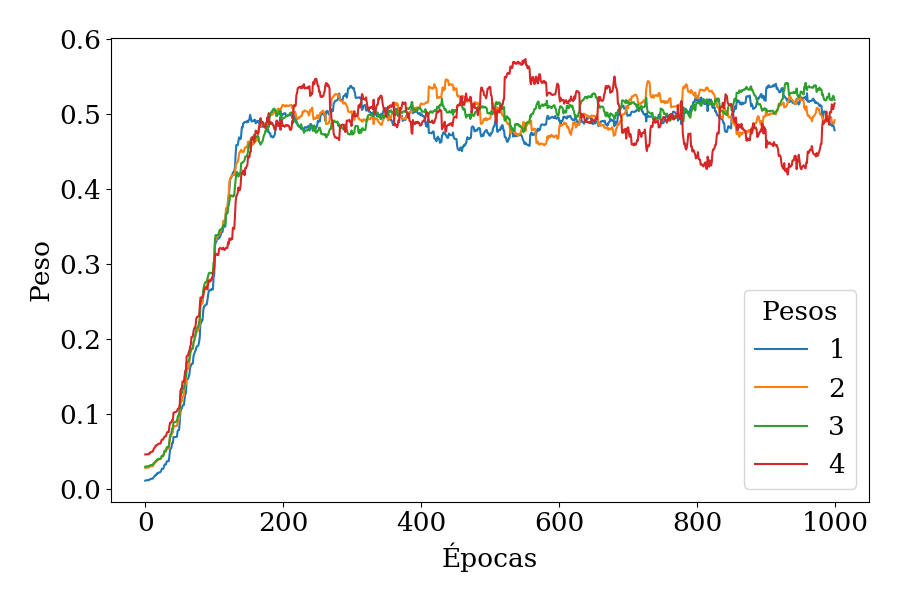
\includegraphics[width=0.45\textwidth]{../Graficos/todos_los_pesos.png}
	\caption{Evolución en función de las épocas de los pesos de la red}
	\label{fig:pesos1D}
\end{figure}

Otro aspecto interesante de la evolución de los pesos, representados como puntos en la Fig.\,\ref{fig:pesos3D}, donde $\bm w$ tiende a alinearse con el vector $\bm \lambda$. Esto se debe a que la dirección predominante en la correlación es la de mayor autovalor, representada por la flecha de línea sólida en la Fig.\,\ref{fig:pesos3D}. Esta figura es una proyección de la espacio de 4 dimensiones, pero tiene la misma apariencia tomando la componente $w_4$ en vez de alguna de las graficadas.
\begin{figure}[H]
	\centering
	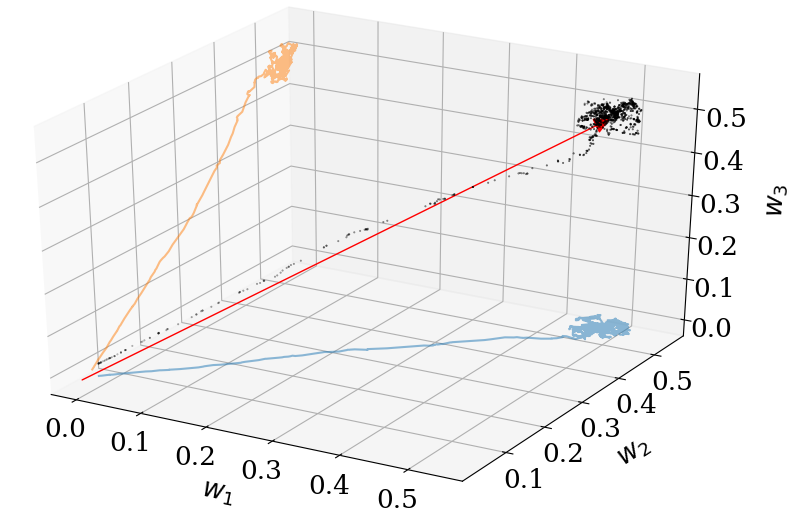
\includegraphics[width=0.5\textwidth]{../Graficos/todos_los_pesos_3D.png}
	\caption{Comparación de los pesos $w_1$, $w_2$ y $w_3$. Se observa los mismos se alinean con la proyección en el esquema tridimensional del autovector con mayor autovalor.}
	\label{fig:pesos3D}
\end{figure}
\section*{Ejercicio 2: Distribución uniforme en un semi-anillo}

La red consiste en una entrada con dos neuronas y una salida de 10 neuronas, donde cada neurona de entrada está conectada a todas las neuronas de salida. Para los datos de entrada tiene una distribución uniforme en un anillo en un rango de $r \in [0.9,1.1]$ y $\theta \in [0,\pi]$, donde $r$ y $\theta$ representan el radio y el ángulo en coordenadas polares. Para obtener una distribución uniforme en el rango considerado, se implementó el siguiente algoritmo:
\begin{align*}
	r^2 &= (\text{random entre 0 y 1})\times(r_{max}^2 - r_{min}^2) + r_{min}^2\\
	\theta &= (\text{otro random entre 0 y 1})\times \pi
\end{align*}
donde $r_{min}=0.9$ y $r_{max}=1.1$. Una vez definido el punto en coordenadas polares, se alimenta a cada neurona de entrada con las coordenadas cartesianas del este punto, mediante la transformación $x = r \cos{\theta} $ e $y = r \sin{\theta}$. La entrada $\bm \xi$ puede tratarse como un vector de dos componentes. La primera entrada es la coordenada x y la segunda es la coordenada y.

Por cada neurona de salida se tiene dos pesos, uno por cada entrada, para un total de 20 valores. Los mismos se organizan como 10 vectores de dos componentes $\bm w_i$, donde la primera componente corresponde al peso de la primera entrada (coordenada x) y lo mismo para la segunda (coordenada y). Los pesos son inicializados tal que la componente en x sea $0.5$ mientras que los valores en $y$ varían entre $(-1.1, 1.1)$.

En cada época, se calcula la salida $O_i$ mediante $O_i = \bm \xi_i \cdot \bm w_i$. Se dice que una neurona de salida $i^*$ es la ganadora cuando $\| \bm \xi - \bm w_{i^*} \|$ tiene el menor valor, en comparación a las otras neuronas $i$. La actualización de los pesos se realiza mediante la Ec.\ref{up_winner}
\begin{equation}
	\Delta w_{i,j} = \eta \Lambda(i, i^*) (\xi_j - w_{i,j})
	\label{up_winner}
\end{equation}
donde $\eta$ en la tasa de aprendizaje y  $\Lambda(i, i^*) $ es la función de inhibición. Para este problema en particular se utilizó la función dada en la Ec.\ref{eq:gauss}, que corresponde a una gaussiana.
\begin{equation}
	\Lambda(i, i^*) = \frac{1}{\sqrt{2\pi}}e^{-\frac{(i-i^*)^2}{2\sigma^2}} \label{eq:gauss}
\end{equation}

La red evolucionó con $\eta=0.02$, además se varió los parámetros $\sigma$ y  $N$, que corresponde a la dispersión de la Ec.\ref{eq:gauss} y la cantidad de épocas.  Se  observaron distintos comportamientos en la convergencia de los pesos para distintos parámetros. En la Fig.\ref{fig:sigma0_6} se observa los pesos iniciales y finales de la red para $\sigma= 0.6$  y distintos tiempos de evolución $N$. La distribución de los datos de entrada se representa con dos arcos concéntricos de radios $0.9$  y $1.1$, centrados en 0. 
\begin{figure}[H]
	\centering
	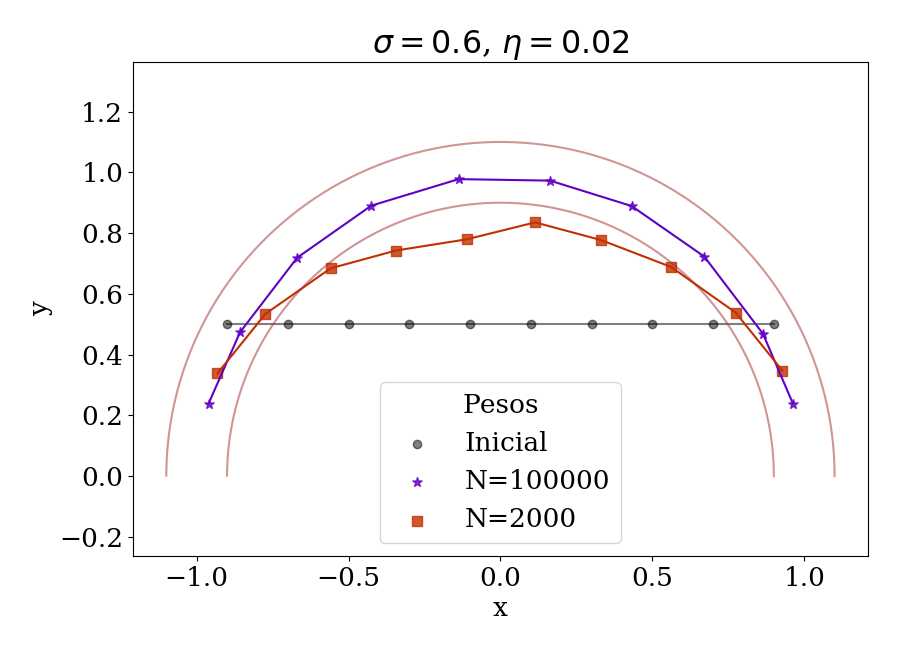
\includegraphics[width=0.5\textwidth]{../Graficos/sigma0_6eta0_02.png}
	\caption{Los valores finales de los pesos para una red con $\sigma=0.6$ y distintas cantidad de épocas. Se puede observar que los pesos copian la distribución de los datos de entrada.}
	\label{fig:sigma0_6}
\end{figure}

Es claro que para $N=1\,000\,000$, los pesos convergen a la distribución de los datos de la entrada, como es de esperarse utilizando el algoritmo de Kohonen, dada por la Ec.\ref{up_winner}, mientras que para $N=2000$ el sistema aún no converge a los valores óptimos.

En cambio si el sistema evoluciona con $\sigma=0.3$, como se muestra en la Fig.\ref{fig:sigma0_3}, para $N=1\,000\,000$, los pesos se distribuyen de forma desordenada, así como también para $N=2000$. Esto se debe a que la función de inhibición inhibe fuertemente a las neuronas lejanas a la neurona ganadora.
\begin{figure}[H]
	\centering
	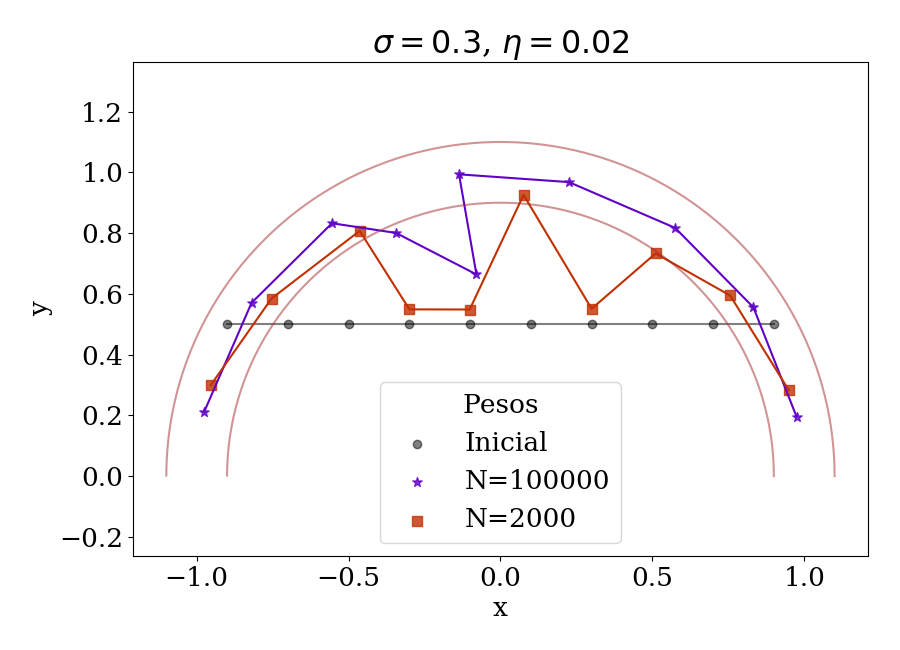
\includegraphics[width=0.5\textwidth]{../Graficos/sigma0_3eta0_02.png}
	\caption{Los valores finales de los pesos para una red con $\sigma=0.3$ y distintas cantidad de épocas.}
	\label{fig:sigma0_3}
\end{figure}


Si relajamos $\sigma$ hasta un valor mayor, como se muestra en la Fig.\ref{fig:sigma2} con $\sigma=2$, el sistema sigue copiando la correlación de los datos de entrada, pero la convergencia se alcanzaría para mayores valores de $N$ en comparación a la Fig.\ref{fig:sigma0_6}.

\begin{figure}[H]
	\centering
	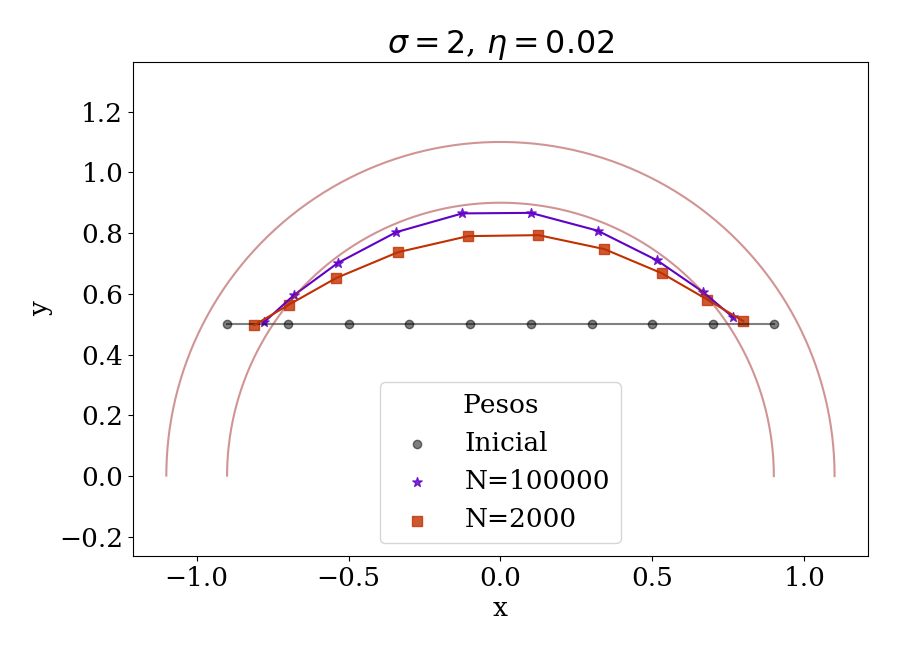
\includegraphics[width=0.5\textwidth]{../Graficos/sigma2eta0_02.png}
	\caption{Los valores finales de los pesos para una red con $\sigma=2$ y distintas cantidad de épocas.}
	\label{fig:sigma2}
\end{figure}

Si seguimos aumentando el valor de $\sigma$, como se muestra en la Fig.\ref{fig:sigma10} con $\sigma=10$, la inhibición ya es débil para forzar a la red a copiar la correlación de los datos de entrada.

\begin{figure}[H]
	\centering
	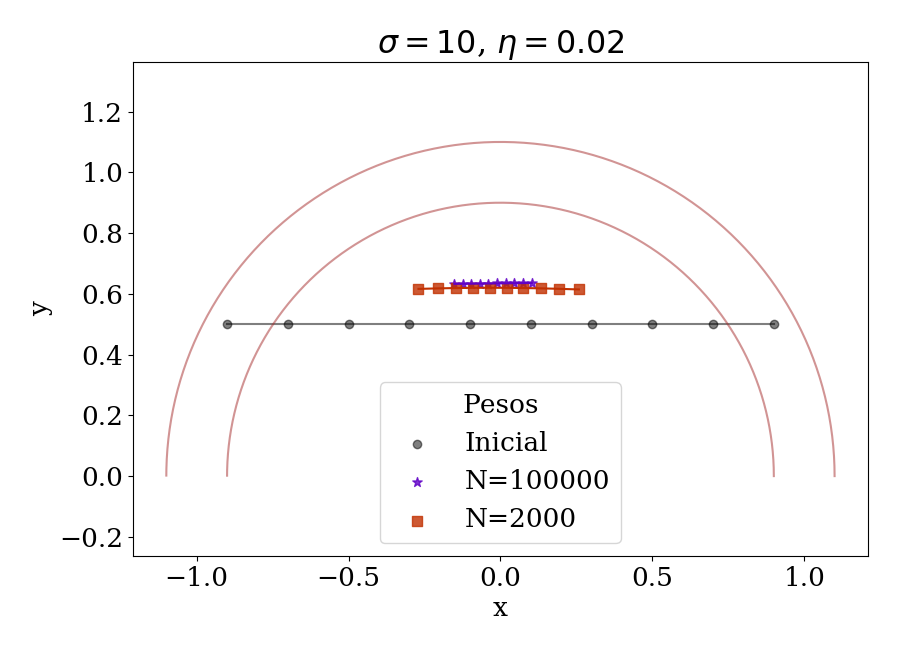
\includegraphics[width=0.5\textwidth]{../Graficos/sigma10eta0_02.png}
	\caption{Los valores finales de los pesos para una red con $\sigma=10$ y distinta cantidad de épocas.}
	\label{fig:sigma10}
\end{figure}


\end{document}